\chapter{L'algorithme RSA en pratique}
    \section{Rappels sur RSA}
        \subsection{Définition}
            \subsubsection{Histoire}
                1976 : Diffie Hellman, New Directions in Cryptography. 1977 : Merkle, "puzzle de Merkle". Rivest, Shamir, Adleman, RSA.

            On fixe $e$ impair ($e = 3, e = 17, e = 257$). On calcule des entiers $p, q$ premiers distincts tels que $\gcd (e, (p-1)(q-1)) = 1$. On pose $n = pq$. Finalement, on calcule $d = e^{-1}[\varphi(n)]$. Clé publique : $(n, e)$. Clé secrète : $(p, q, d, \varphi(n))$.
            \begin{theo}
                Si $p,q$ sont premiers distincts, $n = pq$, $\gcd (e, \varphi(n)) = 1$, $d = e^{-1}[\varphi(n)]$, alors 
                \begin{align*}
                    \begin{array}{cccc}
                        f : & \znz{n} & \to & \znz{n} \\
                        & x & \mapsto & x^e[n] \\
                    \end{array}
                \end{align*}
                est bijective d'inverse
                \begin{align*}
                    \begin{array}{cccc}
                        f^{-1} : & \znz{n} & \to & \znz{n} \\
                        & x & \mapsto & x^d[n] \\
                    \end{array}
                \end{align*}
            \end{theo}
            
        \subsection{Sécurité de RSA}
            Objectif de l'attaquant :
            \begin{enumerate}
                \item Trouver la clé secrète
                \item Calculer $f^{-1}(y)$ pour certains $y$.
            \end{enumerate}
            \begin{itemize}
                \item Trouver $p, q, d, \varphi(n)$ à partir de $n$ et $e$ : déjà, si on connait $p$ ou $q$, on peut facilement retrouver tout le reste de la clé. Ensuite si on connait $\varphi(n) = pq - (p + q) + 1$ et $pq  = n$, donc $p + q = n - \varphi(n) + 1$, $pq = n$, et alors on peut trouver $p, q$. Enfin si on connaît $d$, alors $ed = 1[\varphi(n)]$. Prenons $x$ aléatoire, on calcule $y = x^{\frac{ed - 1}1} [n]$. Et alors $y^2 = x^{ed - 1} = 1[n]$. Mais alors $y$ est solution de l'équation $y^2 = 1 [n]$, qui a $4$ solutions : $(\pm 1, \pm 1) \in \znz{p} \times \znz{q}$ au travers du théorème des restes chinois. Mais alors si $y$ correspond à $(1, -1)$ ou $(-1, 1)$ (notons $\alpha, -\alpha$ les éléments correspondants dans $\znz{n}$), alors $\gcd(y - 1, n) = p$ ou $q$ (vu que $\alpha = 1[p]$ et $\alpha = -1[q]$).
                \item Trouver $f^{-1}(y)$ pour certains $y$ (problème de la racine $e$-ième modulo $n$) : si on sait factoriser, on sait résoudre le problème de la racine $e$-ième grâce au théorème des restes chinois. On ne sait cepandant pas si savoir résoudre le problème des racines $e$-ièmes nous permettrait de résoudre facilement le problème de factorisation. 
            \end{itemize}

    \section{RSA en signature}
        \subsection{Problématique}
            \begin{figure}[H]
                \centering
                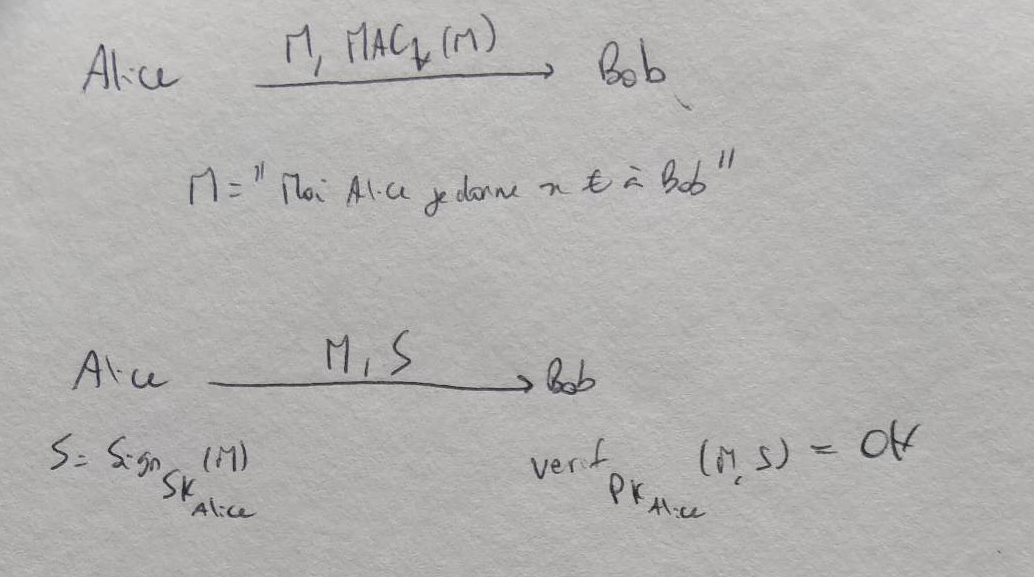
\includegraphics[width=.5\textwidth]{03}
            \end{figure}
            \subsubsection{Algorithme de signature naif}
                On signe avec $f^{-1}(M) = M^d[n]$. Déjà, on doit supposer que $0 \leq M < n$ car sinon on aurait plusieurs messages avec la même signature.
                \begin{itemize}
                    \item Si $M$ est grand, on pourrait écrire $M = \sum M_kn^k$ avec $M_k \in [0, n-1]$, puis on signe par blocs, pas terrible ... 
                    \begin{figure}[H]
                        \centering
                        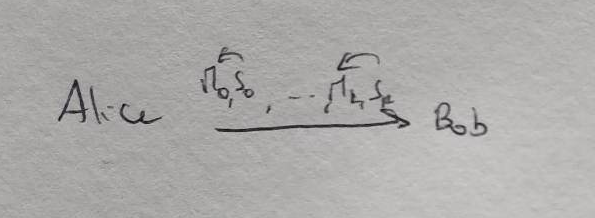
\includegraphics[width=.5\textwidth]{04}
                    \end{figure}
                    \item Problème 2 : Si Alice envoie deux messages signés $(M,S)$ et $(M',S')$, alors charlie peut signer $MM'$ en calculant $SS'$.
                    \item Problème 3 : Si Alice envoie un message $M,S$, alors charlie peut envoyer $M^2, S^2$, $\lambda^eM, \lambda S$.
                    \item Prolbème 4 : charlie peut envoyer $(0, 0)$, $(1, 1)$, $(\lambda^e, \lambda)$.
                \end{itemize}
                
            \subsubsection{Paradigme "hash and sign"}
                \begin{figure}[H]
                    \centering
                    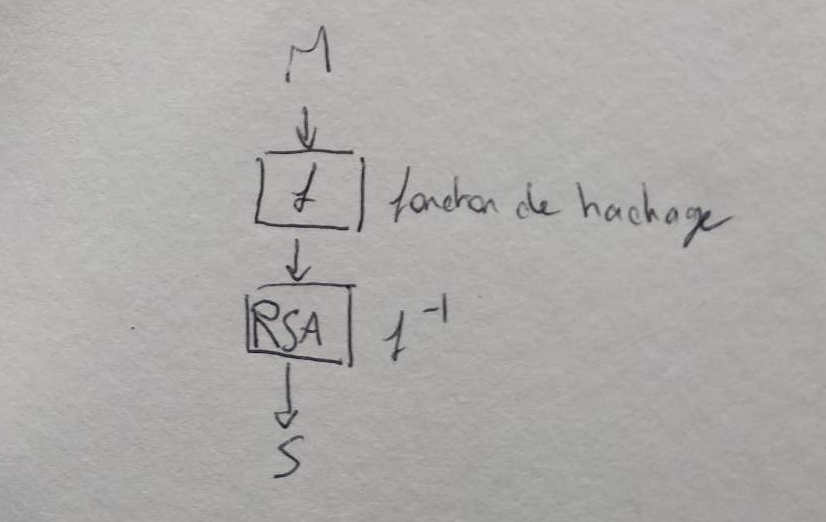
\includegraphics[width=.5\textwidth]{05 }
                \end{figure}

        \subsection{Fonctions de hachage}
            $h : \{0,1\}^* \to \{0,1\}^l$ avec $\{0,1\}^* = \sqcup_{n \geq 0} \{0,1\}^n$ et $l$ un entier fixé. 
            \begin{defi}
                Une telle fonction $h : \{0,1\}^* \to \{0,1\}^l$ est appelée fonction de hachage si elle vérifie les 3 propriétés suivantes : 
                \begin{description}
                    \item[$p_1$ :] $h$ est à sens unique, i.e. pour $y \in \{0,1\}^l$, il est calculatoirement difficile de trouver un antécédent $x$ et $y$. 
                    \item[$p_2$ :] $h$ est à collisions faibles difficiles (second preimage resistant) i.e. pour $x \in \{0,1\}^*$ et $y = h(x)$, il est calulatoirement difficile de trouver $x' \in \{0,1\}$ tel que $x \neq x'$ et $h(x') = y$.
                    \item[$p_3$ :] $h$ est à collisions fortes difficiles (collision resistant) i.e. il est calculatoirement difficile de trouver $x,x' \in \{0,1\}^*$ tel que $x \neq x'$ et $h(x) = h(x')$.   
                \end{description}
            \end{defi}
            \begin{remq}
                $p_2 \Rightarrow p_1$, $p_3 \Rightarrow p_2$. Ainsi d'un point de vu mathématique, $p_3$ suffit, mais il est intéressant de les écrire vu qu'elles ont un intérêt cryptographique.
            \end{remq}
            \begin{enumerate}
                \item Pour la propriété $p_1$, on a un algo qui trouve un antécédent par recherche exhaustive (on tire aléatoirement $x$ et on regarder si $h(x) = y$). La complexité est en $2^l$.
                \item On peut faire la même chose pour la propriété $p_2$. 
                \item On génère aléatoirement $x_1, x_2, \cdots$, et on calcule leurs images $y_i = h(x_i)$ jusqu'à trouver une égalité du type $y_i = y_j$. $P =$ proba d'obtenir une égalité $y_i = y_j$, on peut calculer la probabilité de ne pas avoir de collision $1 - P$.
            \end{enumerate}
            Algorithme pour rechercher des collisions : on fabrique une table de l'ordre de $k \simeq 2^{l/2}$, donc en $\mathcal{O}(k)$, on la trie $\mathcal{O}(k \ln k)$ et la recherche d'une collision est en $\mathcal{O}(k)$. Donc au total une complexité en $\mathcal{O}(l2^{l/2})$. Ainsi on doit prendre $l \geq 256$.

        \subsection{Exemple : la fonction de hachage de Chaum-van Heijst-Pfitzmann}
            Soit $p$ un nombre premier tel que $q = \frac{p - 1}2$ est aussi premier, $g,h$ deux éléments d'ordre $q$ dans $\znz{p}^*$. On définit 
            \begin{align*}
                \begin{array}{cccc}
                    H : & \znz{q} \times \znz{q} & \to & \znz{p}^* \\
                    & (m_1, m_2) & \mapsto & g^{m_1} h^{m_2} \\
                \end{array}
            \end{align*}
            (Ce n'est pas à proprement parler une fonction de hachage vu l'ensemble de départ, mais une fonction de compression). 
            \begin{description}
                \item[Quelle est l'image de $H$ ?] Considérons $A = \bra g \ket$, $B = \bra h \ket$, et $C = \{u \in \znz{p}^* \mid u^q = 1\}$. Alors $A \subseteq C$, $B \subseteq C$, et $\card{C} \leq q = \card{A} = \card{B}$, donc au final $A = B = C$. Et finalement si $y \in A = B = C$, il existe $t \mid y = g^t$ donc $y = H(t, 0)$ et ainsi $A \subseteq \im H$ (l'inclusion réciproque est claire).
                \item[Supposons que Charlie trouve une collision : ] $H(m_1, m_2) = H(m_3, m_4)$ avec $(m_1, m_2) \neq (m_3, m_4)$. Alors
                \begin{align*}
                    g^{m_1}h^{m_2} = g^{m_3}h^{m_4} \iff g^{m_1 - m_3} = h^{m_4 - m_2}
                \end{align*} 
                Posons $d = \gcd (m_4 - m_2, p - 1) \in \{1, 2, q, p - 1\}$, alors
                \begin{itemize}
                    \item Si $d = 1$, $m_4 - m_2$ a une inverse $w$ modulo $p - 1$, et alors
                    \begin{align*}
                        g^{(m_1 - m_3)} = h^{(m_4 - m_2)w} = h
                    \end{align*}
                    \item Si $d = 2$, alors $\gcd(m_4 - m_2, q) = 1$. Notons alors $\theta$ l'inverse de $m_4 - m_2$ modulo $q$, alors
                    \begin{align*}
                        g^{(m_1 - m_3)\theta} = g^{(m_4 - m_2)\theta} = h
                    \end{align*}
                    \item Si $d = q$, alors $q \mid m_4 - m_2$, donc $m_2 = m_4$. Ainsi $g^{m_1 - m_3} = 1[p]$, donc $q \mid m_1 - m_3$ et donc $m_1 = m_3$, donc les deux messages sont égaux, absurde.
                    \item Si $d = p - 1$, de même $q \mid m_4 - m_2$ ... 
                \end{itemize}
                Ainsi savoir trouver une collision de cette fonction de hachage implique que l'on sait résoudre le problème du log discret. Ainsi réciproquement si on trouve $g$ et $h$ tels que le problème du log discret est difficile avec, alors il sera difficile de trouver une collision pour cette fonction de hachage.
            \end{description}
            
        \subsection{Construction de Merkle-Damgard}
            En chiffrement symétrique, si on veut chiffrer un gros bloc $x = x_1 x_2 \cdots x_k$, on disposes de modes d'opérations pour chiffrer ces blocs : on peut par exemple chiffrer chaque bloc les uns après les autres (ECB). On peut aussi utiliser le mode CBC. \\
            Hypothèse : $f : \{0,1\}^m \to \{0,1\}^l$ est une fonction de compression ($m > l + 1$). Peut-on fabriquer une fonction de hachage à partir de cette fonction de compression ? Soit $x \in \{0, 1\}^*$, on le découpe en blocs $x = x_1 \| x_2 \| \cdots \| x_k$, en blocs de $m - l - 1$ bits pour les $k - 1$ premiers blocs, et le dernier bloc est de taille $\leq m - l - 1$. On définit ensuite $y = y_1 \| y_2 \| \cdots \| y_k \| y_{k + 1}$ avec $y_i = x_i$ pour tout $1 \leq i \leq k - 1$, et $y_k = x_k \| 0 \cdots 0$ est la complétion de $x_k$ avec des zéros (disons $d$) pour faire $m - l - 1$ bits. Finalement on pose $y_{k + 1} = d$ (son écriture binaire). Finalement on hash $y$ de la manière suivante :
            
            \begin{figure}[H]
                \centering
                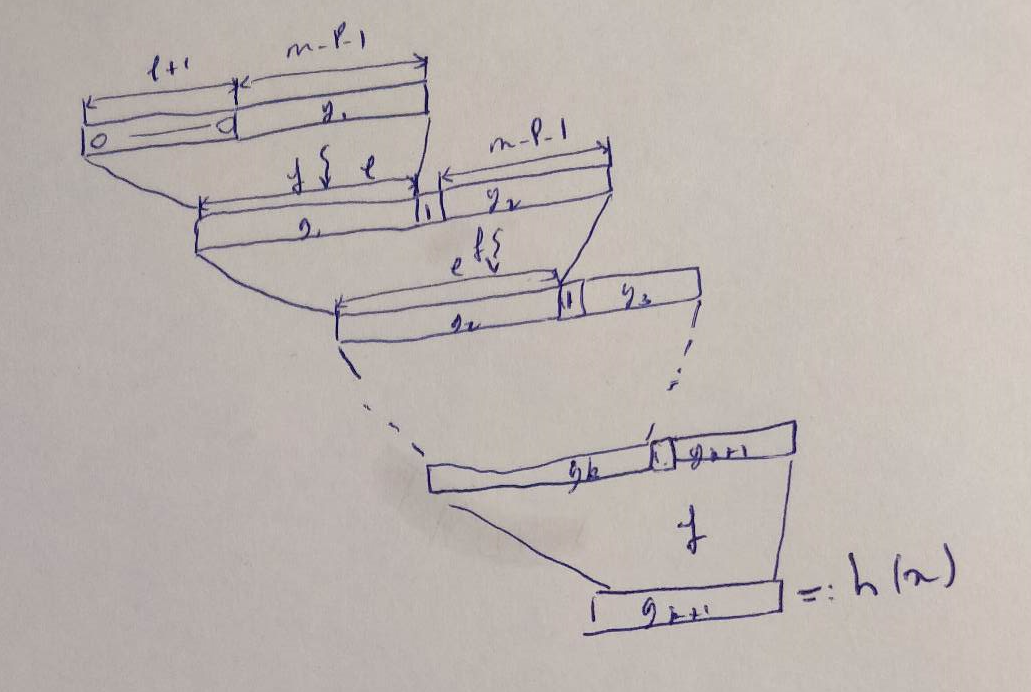
\includegraphics[width=.7\textwidth]{06}
            \end{figure} \noindent

            \begin{theo}
                Si $f$ est à collision fortes difficiles, alors $h$ aussi.
            \end{theo}
            \begin{proof}
                Supposons qu'on ai une collision $h(x) = h(x')$ avec $x \neq x'$. $x,x'$ correspondent à $y,y'$ par la construction décrite précédemment. Remarquons alors qu'au vu de la construction, $y \neq y'$. Notons $k,t$ le nombre de blocs de $x,x'$ (donc $y,y'$ ont $k + 1, t + 1$ blocs). Ainsi avec les notations de la figure précédente, $g_{k + 1} = g'_{t + 1}$, i.e. $f(g_k \| 1 \| y_{k + 1}) = f(g'_t \| 1 \| y'_{t + 1})$.
                \begin{itemize}
                    \item Si $y_{k + 1} \neq y'_{t + 1}$, alors on obtiens une collision pour $f$.
                    \item Si $g_k \neq g'_t$, alors on obtiens aussi une collision pour $f$.
                    \item Si $g_k = g'_t$ et $y_{k + 1} = y'_{t + 1}$, alors $f(g_{k - 1} \| 1 \| y_k) = f(g'_{t - 1} \| 1 \| y'_t)$, et on réapplique le point précédent. On peut alors soit trouver une collision dans ce procédé, soit remonter complètement la construction de $h$. Il y a alors trois cas : soit on remonte la construction pour $y$ mais pas pour $y'$, (donc $k < t$), alors $g_1 = g'_{t - k + 1}$, ainsi $f(0 \cdots 0 \| y_1) = f(g'_{t - k} \| 1 \| y'_{t - k + 1})$, donc on obtiens une collision. De même si on remonte la construction pour $y'$ mais pas pour $y$. Et finalement si on remonte les deux constructions en même temps, alors $f(0 \| y_1) = f(0 \| y'_1)$, alors si $y_1 \neq y'_1$, on obtiens une collision, et sinon $y = y'$ et donc $x = x'$, contradiction.
                \end{itemize}
            \end{proof}
            
            \subsubsection{Attaque de Bleichenbacher}
                \begin{description}
                    \item[Hypothèses :] 
                    \begin{itemize}
                        \item $h$ fonction de hachage construite avec Merkle-Damgard
                        \item On dispose d'une collision $M$ et $M'$ avec $h(M) = H(M')$ et $M \neq M'$.
                    \end{itemize}
                    \item[Objectif :] l'attaquant choisit deux textes $T$ et $T'$. Problème : construire deux fichiers $F$ et $F'$ tels que $F$ affiche $T$, $F'$ affiche $T'$, et $h(F) = h(F')$.
                \end{description}
                Fichiers postscript .ps :
                
                \begin{figure}[H]
                    \centering
                    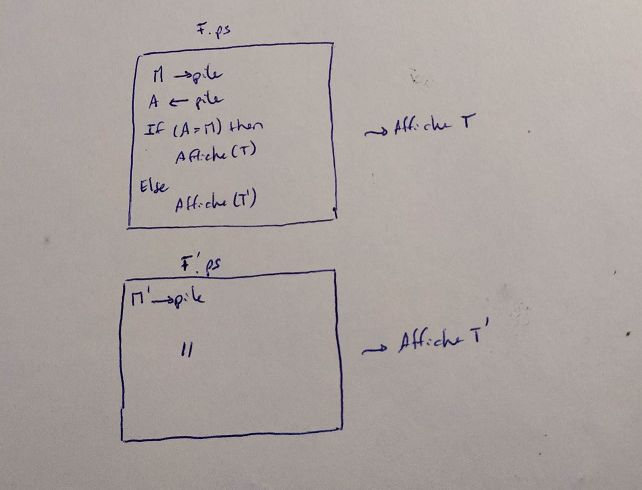
\includegraphics[width=.7\textwidth]{07}
                \end{figure} \noindent
                
                Mais comme $M$ et $M'$ collisionnent, alors le haché de ces deux fichiers est le même et on a bien obtenu ce que l'on voulait.

        \subsection{Fonctions de hachage usuelles}
            \begin{tabular}{c|c|c|c|c|c}
                Nom & Année & Inventeurs & $l$ & Anniv & Meilleure attaque connue \\
                \hline
                MD4 & 1990 & Rivest & $128$ & $2^{64}$ & 1995, Dobbertim trouve une collision \\
                \hline
                MD5 & 1991 & Rivest & $128$ & $2^{64}$ & 2005, Wang : plusieurs collisions en $2^{24}$\\
                \hline
                SHA{\color{blue}-0} & 1993 & NIST & 160 & $2^{80}$ & 2004, Joux : collision en $2^{51}$ \\
                \hline
                SHA-1& 1994 & NIST & $160$ & $2^{80}$ & 2006, Wang : algo pour trouver \\
                &&&&& des collisions en $2^{69}$. En $2016$, \\
                &&&&& Stevens, ... trouvent une collision \\
                \hline
                {\color{blue} Famille SHA-2}& 2002 & NIST & 256 & $2^{128}$ & $\emptyset$ \\
                SHA-256 &&& 384 & $2^{192}$& \\
                SHA-384 &&& 512 & $2^{256}$& \\
                SHA-512 &&&&& \\
                \hline
                SHA-3 & 2011 & Bertoni, Daemen, & 224 & $2^{112}$ & $\emptyset$ \\
                && Peters, van Asche & 256 & $2^{128}$ &\\
                && (KECCAK) & 384 & $2^{192}$ &\\
                &&& 512 & $2^{256}$ &\\
            \end{tabular}

        \subsection{Standards de signature RSA}
            Pour signer avec RSA, on réalise $s = (\mu(M))^d [n]$ où $\mu$ est un standard de signature RSA. 
            \begin{expl}
                PKCS (RSA DATA Security), Public Key Cryptographic Standard, propose (PKCS 1 v1.7) 
                \begin{align*}
                    \mu(M) = 00 \| 01 \| FF \cdots FF \| 00 \| c_h \| h(M) < n
                \end{align*}
                où $c_h$ est le numéro de la fonction de hachage.
            \end{expl}
            \begin{expl}
                ISO 9796-2 : on découpe $M = M_1 \| M_2$ de sorte que  
                \begin{align*}
                    \mu(M) = 6A \| M_1 \| h(M) \| BC < n
                \end{align*}
                Alice envoie alors $M_2$ et la signature (Bob peut alors récupérer $M_1$ dans la signature).
            \end{expl}
            
    \section{RSA en chiffrement}
        \subsection{Théorème de Coppersmith}
            \begin{theo} (Coppersmith, 1997)
                $N$ entier, $f \in \mathbb{Z}[X]$ polynôme unitaire de degré $d$. Posons $B = N^{\frac 1d - \varepsilon}$ ($\varepsilon > 0$), alors étant donné $f$ et $N$, on peut trouver efficacement tous les entiers $x_0$ tels que $|x_0| < B$ et $f(x_0) = 0 [N]$.
            \end{theo}
            Or si on chiffre $C = M^e [N]$, cela revient à résoudre le polynôme $f(x) = x^e - C$. Et dans ce cas, si $M < N^{\frac 1e}$, alors $M^e < N$ et donc $C = M^e$, d'où $M = {}^e\sqrt{C}$. \\
            Pour la démonstration, nous aurons besoin d'un lemme. Pour cela, soit $h(x) = \sum a_i x^i \in \mathbb{Z}[X]$, alors on pose $\|h\|^2 = \sum |a_i|^2$. On note $h(B \cdot)$ le polynôme $h(BX)$. Alors on a
            \begin{lemm}
                Pour $h \in \mathbb{Z}[X]$ de degré $d$ et $B > 0$ entier, supposons que $\|h(B \cdot) \| < \frac{N}{\sqrt{d + 1}}$ et si $|x_0| < B$ satisfait $h(x_0) = 0 [N]$, alors $h(x_0) = 0$.
            \end{lemm}
            \begin{proof}
                \begin{align*}
                    |h(x_0)| &= \left| \sum a_i x_0^i \right| = \left| \sum a_i \frac{x_0^i}{B^i}B^i \right| \\
                    &\leq \sum \left| a_i \frac{x_0^i}{B^i}B^i \right| \leq \sum \left| a_i B^i \right| \\
                    &\leq \sqrt{d + 1} \|h(B \cdot) \| < N \\
                \end{align*}
                Et ainsi $h(x_0) = 0$.
            \end{proof}
            L'idée de Coppersmith est de considérer la famille 
            \begin{align*}
                g_{u, v}(x) = N^{m - v} x^u f(x)^v
            \end{align*}
            Si $x_0$ est racine de $f$ modulo $N$, alors $x_0$ est racine de $g_{u, v}$ modulo $N^m$. En effet, on peut alors écrrie $f(x_0) = \lambda N$, et alors $N^{m - v} x_0^u \lambda^v N^v = 0[N^m]$. On va prendre les $g_{u, v}$ poru $u = 0, 1, \cdots, d - 1$, et $v = 0, \cdots, m$. Mettons brièvement en pause la démonstration pour parler de réseaux.

            \subsubsection{Réseaux euclidiens}
                \begin{defi}
                    Soit $u_1, u_2, \cdots, u_w \in \mathbb{Z}^w$ \cor{Entiers ou réels ? peut-être peu importe pour la suite} des vecteurs linéairement indépendants. On appelle réseau $L$ engendré par $u_1, \cdots, u_w$ l'ensemble des combinaisons linéaires à coefficients entiers des $u_1, \cdots, u_w$.
                \end{defi}
                \begin{defi}
                    Le déterminant de $L$ est le déterminant de la matrice dont les lignes sont les vecteurs $u_1, \cdots, u_w$.
                \end{defi}
                \begin{theo} (Hermite)
                    Tout réseau $L$ de dimension $w$ contient un vecteur $v \in L \bs \{0\}$ dont la norme vérifie $\|v\| \leq \gamma_w (\det L)^{\frac 1w}$.
                \end{theo}
                Algorithme LLL (Lovasz, A. Lenstra, H. Lenstra, 1982) : étant donné $L$ un réseau engendré par les vecteurs $u_1, \cdots, u_w$, l'algorithme renvoie un vecteur $v$ non nul du réseau tel que $\|v\| < 2^{\frac w4} (\det L)^{\frac 1w}$ en temps polynomial.

            Revenons au problème initial :
            \begin{expl}
                $m = 3$, $d = 2$,
                \begin{align*}
                    \begin{array}{c||c|c|c|c|c|c|c|c}
                        & 1 & X & X^2 & X^3 & X^4 & X^5 & X^6 & X^7 \\
                        \hline
                        g_{0, 0}(BX) & N^3 & & & & & & & \\
                        g_{1, 0}(BX) & & BN^3 & & & & & & \\
                        g_{0, 1}(BX) & & & B^2N^2 & & & & & \\
                        g_{1, 1}(BX) & & & & B^3N^2 & & & & \\
                        g_{0, 2}(BX) & & & & & B^4N & & & \\
                        g_{1, 2}(BX) & & & & & & B^5N & & \\
                        g_{0, 3}(BX) & & & & & & & B^6 & \\
                        g_{1, 3}(BX) & & & & & & & & B^7 \\
                    \end{array}
                \end{align*}
                Ainsi $\det L$ est le produit des termes sur la diagonale.
            \end{expl}
            Plus généralement,
            \begin{align*}
                \det L = \prod_{u = 0}^{d - 1} \prod_{v = 0}^m N^{m - v} B^{vd + u}
            \end{align*}
            On veut trouver $m$ tel que $2^{\frac w4} (\det L)^{\frac 1w} < \frac{N^m}{\sqrt{w}}$, alors on pourra trouver un vecteur $v$ tel que $\|v\| \leq \frac{N^n}{\sqrt{w}}$ en utilisant l'algo LLL (on sera alors dans les conditions du lemme)
            \begin{align*}
                \det L &= \prod_{u = 0}^{d - 1} B^{(m + 1)u} \prod_{v = 0}^m N^{m - v}B^{vd} \\
                &= N^{d \frac{m(m + 1)}2} \prod_{u = 0}^{d - 1} B^{(m + 1)u} \prod_{v = 0}^m B^{vd} \\
                &= N^{d \frac{m(m + 1)}2} \prod_{u = 0}^{d - 1} B^{(m + 1)u} B^{d \frac{m(m + 1)}2} \\
                &= N^{d \frac{m(m + 1)}2} B^{d^2 \frac{m(m + 1)}2} \prod_{u = 0}^{d - 1} B^{(m + 1)u}  \\
                &= N^{d \frac{m(m + 1)}2} B^{d^2 \frac{m(m + 1)}2} B^{(m + 1) \frac{d(d - 1)}2} \\
                &= N^{d \frac{m(m + 1)}2} B^{\frac{d(m + 1)}2 (dm + d - 1)} \\
                &= N^{\frac{dm(m + 1)}2} B^{\frac{d(m + 1)}2 (d(m + 1) - 1)} \\
            \end{align*}
            Et donc il suffit de trouver $m$ tel que
            \begin{align*}
                2^{\frac{d(m + 1)}4} N^{\frac m2} B^{\frac{d(m + 1) - 1}2} < \frac{N^m}{\sqrt{d(m + 1)}}
            \end{align*}
            Mais
            \begin{align*}
                2^{\frac{d(m + 1)}4} N^{\frac m2} B^{\frac{d(m + 1) - 1}2} < \frac{N^m}{\sqrt{d(m + 1)}} &\iff B < \alpha(d, m) N^{\frac m{d(m + 1) - 1}}  < N^{\frac 1d - \varepsilon} \\
            \end{align*}
            pour $m$ assez grand. 

        \subsection{Attaque de Hastad}
            \begin{figure}[H]
                \centering
                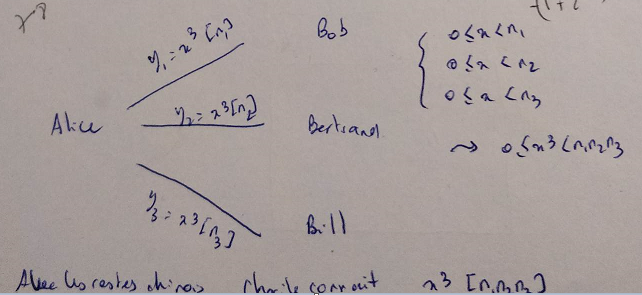
\includegraphics[width=.7\textwidth]{08}
            \end{figure} \noindent

            Piste de réparation : l'utilisateur numéro $i$ publie $N_i$, $e_i$ (son modulo et son exposant publique), et $f_i \in \znz{N_i}[x]$, et il envoie $(f(M_i))^{e_i} [N_i]$. 
            \begin{theo} (Attaque de Hastad améliorée)
                \begin{itemize}
                    \item $N_1, \cdots, N_k$ entiers premiers entre eux $2$ à $2$
                    \item On pose $N_{\min} = \min_{1 \leq i \leq k} N_i$
                    \item $g_i \in \znz{N_i} [X] (1 \leq i \leq k)$ : $k$ polynômes de degré maximum $d$
                \end{itemize}
                S'il existe un unique $M < N_{\min}$ tel que $\forall 1 \leq i \leq k, g_i(M) = 0 [N_i]$, et si $k \geq d$, alors on peut trouver $M$ en temps polynomial.
            \end{theo}
            \begin{proof}
                Notons $\overline{N} = N_1N_2 \cdots N_k$.
                \begin{itemize}
                    \item On peut supposer les $g_i$ unitaires (si ce n'est pas possible, on peut factoriser $N_i$ par un pgcd du coefficient dominant de $g_i$).
                    \item On suppose que tous les $g_i$ sont de degré $d$ (quitte à multiplier par une puissance de $X$)
                    \item On définit le polynôme
                    \begin{align*}
                        g(x) = \sum_{i = 1}^k T_i g_i(x) \in \znz{\overline{N}}[X]
                    \end{align*}
                    avec $T_i = 1 [N_i]$ et $T_i = 0 [N_j]$ pour tout $j \neq i$.
                \end{itemize}
                $g$ est unitaire de degré $d$, $g(M) = 0 [\overline{N}]$, $M < N_{min} \leq \overline{N}^{\frac 1k} \leq \overline{N}^{\frac 1d}$. Ainsi d'après le théorème de Coppersmith, on trouve $M$ en temps polynomial. 
            \end{proof}

        \subsection{Short pad attack}
            \begin{description}
                \item[Idée :] pour chiffrer $M$, on calcule $C = (2^mM + r)^e [N]$ (où $M$ es le message clair, d'au plus $k - m$ bits, et $r$ fait $m$ bits). Cela rebient à chiffrer la concatenation $M \| r$.
                \item[Attaque (Coppersmith) :] $(N, e)$ clé publique de RSA, $N$ de taille $k$ bits, $m = \lfloor \frac k{e^2} \rfloor$. Supposons que l'attaquent récupère deux chiffrés de $M$ $C_1 = M_1^e [N]$ avec $M_1 = 2^mM + r_1$, $C_2 = M_2^e [N]$ avec $M_2 = 2^mM + r_2$. On définit $g_1(x, y) = x^e - c_1$, $g_2(x, y) = (x + y)^e - c_2$. Quand $y = r_2 - r_1$, alors $M_1$ est une racine commune pour $g_1(\cdot, y)$ et $g_2(\cdot, y)$. Soit $h(y) = Res_x(g_1, g_2)$. Alors $h(y) = 0$ quand $y = r_2 - r_1$... ff
            \end{description}

    \section{Attaques physiques}
        \subsection{Carte à puce}
            \cor{FIGURE 1}

        \subsection{Attaque SPA}
            Paul Kocher, 1998.
            \cor{FIGURE 2}
            % \def\scl{0.6}%scaling factor of the picture
            % \begin{tikzpicture}[
            % scale=\scl,
            % controlpanels/.style={yellow!30!brown!20!,rounded corners,draw=black,thick},
            % screen/.style={green!50!black!60!,draw=black,thick},
            % trace/.style={green!60!yellow!40!, ultra thick},
            % smallbutton/.style={white,draw=black, thick},
            % axes/.style={thick}]
            % \fill[green!30!blue!30!,rounded corners,draw=black,thick](0,0)
            %     rectangle (27.75,13.25);
            % \fill[fill=black!40!,draw=black,thick,rounded corners](0.25,0.25)
            %     rectangle (27.5,13.00);
            % % Screen, centered around the origin then shifted for easy plotting
            % \begin{scope}[xshift=7cm,yshift=8cm,samples=150]
            %     \fill[black!60!,rounded corners,draw=black,thick](-5.3,-4.3)
            %     rectangle (5.3,4.3);
            %     \fill[screen] (-5.0,-4.0) rectangle (5.0,4.0);
            %     \draw[trace] plot(\x,{1+2.4*sin((2.5*\x +1) r)}); % r for radians...
            %     \draw[trace] plot(\x,{-1+1.25*sin((0.75*\x) r});
            %     \draw[thin] (-5.0,-4.0) grid (5.0,4.0);
            %     \draw[axes] (-5,0)--(5,0); % Time axis
            %     \draw[axes] (0,-4)--(0,4);
            %     \foreach \i in {-4.8,-4.6,...,4.8} \draw (\i,-0.1)--(\i,0.1);
            %     \foreach \i in {-3.8,-3.6,...,3.8} \draw (-0.1,\i)--(0.1,\i);
            % \end{scope}
            % % Feet
            % \fill[black!70!,rounded corners,xshift=2cm] (0,-.5) rectangle (2,0);
            % \fill[black!70!,rounded corners,xshift=23.75cm] (0,-.5) rectangle (2,0);
            % % Lower left panel
            % \fill[controlpanels] (0.6,0.5) rectangle (13.5,3.0);
            % \path (0.8,0.9) node[scale=\scl,right]{$\mathbf{TeXtronics\,1 - v.1.01}$};
            % % Lower right panel
            % \fill[controlpanels] (13.7,0.5) rectangle (27.1,6.2);
            % %Channels
            % % CH I
            % \draw[thick] (14.8,1.5) circle (0.7cm);
            % \fill[gray,draw=black,thick] (14.8,1.5) circle (0.5cm);
            % \fill[white,draw=black,thick] (14.8,1.5) circle (0.3cm);
            % \node[scale={1.5*\scl}] at (14.8,2.5) {CH I};
            % \draw[thick] (16.2,1.5) circle (0.4cm);
            % \fill[black!60!] (16.2,1.5) circle (0.3cm);
            % \draw[thick] (16.6,1.5) --(17,1.5)--(17,1.0);
            % \draw[thick] (16.7,1.0)--(17.3,1.0);
            % \draw[thick] (16.8,0.85)--(17.2,0.85);
            % \draw[thick] (16.9,0.70)--(17.1,0.70);
            % \draw[thick] (26.0,1.5) circle (0.7cm);
            % % CH II
            % \fill[gray,draw=black,thick] (26,1.5) circle (0.5cm);
            % \fill[white,draw=black,thick] (26,1.5) circle (0.3cm);
            % \node[scale={1.5*\scl}] at (26,2.5) {CH II};
            % \draw[thick] (24.6,1.5) circle (0.4cm);
            % \fill[black!60!] (24.6,1.5) circle (0.3cm);
            % \draw[thick] (24.2,1.5) --(23.7,1.5)--(23.7,1.0);
            % \draw[thick] (23.4,1.0)--(24.0,1.0);
            % \draw[thick] (23.5,0.85)--(23.9,0.85);
            % \draw[thick] (23.6,0.70)--(23.8,0.70);
            % \draw[thick] (26.0,1.5) circle (0.7cm);
            % % Y-pos
            % \fill[smallbutton] (14.8,4.9) circle (0.3cm);
            % \node[scale={\scl}] at (14.8,5.5) {Y-pos I};
            % \fill[smallbutton] (26.0,4.9) circle (0.3cm);
            % \node[scale={\scl}] at (26.0,5.5) {Y-pos II};
            % % Volt/div the foreach loop draws the two buttons
            % \foreach \i / \b in {18/75,22.5/345}{
            % %Second parameter of the loop is the angle of the index mark 
            % \begin{scope}[xshift=\i cm,yshift=3.8cm,scale=0.85]
            %     \node[scale=\scl] at (0,2.3) {Volts/Div};
            %     \node[scale=\scl,black] at (-1,-2.4) {V};
            %     \node[scale=\scl,blue]  at (1,-2.4) {mV};
            %     \clip[rounded corners] (-2,-2) rectangle (2,2);
            %     \fill[black!30!,rounded corners,draw=black,thick] (-2,-2)
            %     rectangle (2,2);
            %     \fill[blue!50!black!20!,draw=black,thick]
            %     (30:1.1)--(30:3)--(3,-3)--(-90:3)--(-90:1.1) arc (-90:30:1.1);
            %     \draw[very thick,rounded corners](-2,-2) rectangle (2,2);
            %     \draw[thick] (0,0) circle (1.0);
            %     \foreach \i in {0,30,...,330}
            %     \draw[thick] (\i:1.2)--(\i:2.5);
            %     \foreach \i/\j in {15/50,45/.1,75/.2,105/.5,135/1,165/2,195/5,225/10,
            %     255/20,285/5,315/10,345/20} \node[scale=\scl,black] at (\i:1.7) {\j};
            %     \fill[blue!30!black!60!,draw=black,thick] (0,0) circle (0.8cm);
            %     % Here you set the right Volts/Div button
            %     \draw[ultra thick,red] (\b:0.3)--(\b:1.2);
            % \end{scope}}
            % % Upper right panel
            % \fill[controlpanels] (13.7,6.5) rectangle (27.1,12.75);
            % %On-Off button
            % \draw[rounded corners,thick,blue] (13.9,10.5) rectangle (15.9,12.5);
            % \fill[fill=red,draw=black,thick,rounded corners] (14.4,10.8) rectangle (15.3,11.2);
            % \node[scale=\scl] at (14.8,12) {\textbf{Power}};
            % \node[scale=\scl] at (14.8,11.5) {\textbf{On/Off}};
            % % Focus-Intensity buttons
            % \draw[rounded corners,thick,blue] (13.9,7.0) rectangle (15.9,10.0);
            % \fill[smallbutton] (14.9,7.5) circle (0.3cm);
            % \node[scale=\scl] at (14.9,8.2) {\textbf{Focus}};
            % \fill[smallbutton] (14.9,9) circle (0.3cm);
            % \node[scale=\scl] at (14.9,9.6) {\textbf{Intens}};
            % % X-pos
            % \fill[smallbutton] (24.5,9.9) circle (0.3cm);
            % \node[scale={\scl}] at (24.5,10.5) {X-pos};
            % % Time/Div
            % \begin{scope}[xshift=21cm,yshift=9.5cm,scale=1]
            %     \node[scale={1.25*\scl}]  at (0,2.4) {Time/Div};
            %     \clip[rounded corners] (-2.2,-2) rectangle (2.2,2);
            %     \fill[black!30!,rounded corners,draw=black,thick] (-2.2,-2) rectangle (2.2,2);
            %     \fill[blue!50!black!20!,draw=black,thick]
            %     (45:1.1)--(45:3)--(3,-3)--(-90:3)--(-90:1.1) arc (-90:45:1.1);
            %     \fill[green!50!black!40!,draw=black,thick]
            %     (45:1.1)--(45:3) arc(45:207:3) --(207:1.1) arc (207:45:1.1);
            %     \draw[very thick,rounded corners](-2.2,-2) rectangle (2.2,2);
            %     \node[scale={1.25*\scl}] at (-1.6,-1.6) {$s$};
            %     \node[scale={1.25*\scl}] at (1.6,-1.6) {$\mu{}\,s$};
            %     \node[scale={1.25*\scl}] at (-1.6,1.6) {$m\,s$};
            %     \draw[thick] (0,0) circle (1.0);
            %     \foreach \i in {-72,-54,...,262} \draw[thick] (\i:1.15)--(\i:1.35);
            %     \foreach \i/\j in {-72/.5,-54/1,-36/2,-18/5,0/10,18/20,36/50,54/.1,72/.2,90/.5,
            %     108/1,126/2,144/5,162/10,180/20,198/50,216/.1,234/.2,252/.5}
            %     \node[scale=\scl,black] at (\i:1.7){\j};
            %     \fill[blue!30!black!60!,draw=black,thick] (0,0) circle (0.8cm);
            %     % Here you set the Time/Div button
            %     \draw[ultra thick,red] (-18:0.3)--(-18:1.2);	
            %     % X-pos
            % \end{scope}
            % \end{tikzpicture}
            Square and multiply always : on fait multiply à chaque itération de l'algo.

        \subsection{Timing attack}
            \cor{FIGURE 3}
            \begin{description}
                \item[Hypothèse :] le calcul de $a \times b [n]$ prends un temps $\alpha$ ou $\beta > \alpha$ (par exemple la multiplication modulaire de Montgomery). 
                \item[Question :] On réalise square and multiply always, la question étant a-t-on calculé $x^6*x [n]$ ? 
                \begin{align*}
                    A &= \{1 \leq i \leq n \mid x_i^6 \times x_i [n] \text{ prends un temps } \alpha\} \\
                    B &= \{1 \leq i \leq n \mid x_i^6 \times x_i [n] \text{ prends un temps } \beta\} \\
                    T_A &= \frac{1}{\card{A}} \sum_{i \in A} T_i \\
                    T_B &= \frac{1}{\card{B}} \sum_{i \in B} T_i \\
                \end{align*}
                Pour $i \in A$, $T_i =$temps$(x_i^6 \times x_i) +$ autre temps. Pareil pour $i \in B$. Donc
                \begin{align*}
                    T_A &= \alpha + \frac{1}{\card{A}} \sum_{i \in A} \text{bruit} \\
                    T_A &= \beta + \frac{1}{\card{B}} \sum_{i \in B} \text{bruit} \\
                \end{align*}
                Ainsi $T_b - T_a = \beta - \alpha + \mathcal{O} \left(\frac 1{\sqrt{\card{A}}} + \frac 1{\sqrt{\card{B}}} \right)$ si $x^6 \times x$ existe, sinon seulement $\mathcal{O} \left(\frac 1{\sqrt{\card{A}}} + \frac 1{\sqrt{\card{B}}} \right)$. Cela nous permet de savoir si le calcul a été réalisé, et on peut donc de proche en proche déduire la marche de l'algorithme square and multiply
            \end{description}

        \subsection{Attaque DPA (Differential Power Analysis)}
            \cor{FIGURE 4}
            \begin{align*}
                A &= \{1 \leq i \leq N,\, \text{le bit de poids fort de } x_i^6 \times x_i [n] \text{ vaut } 0\} \\
                B &= \{1 \leq i \leq N,\, \text{le bit de poids fort de } x_i^6 \times x_i [n] \text{ vaut } 1\} \\
                \mathcal{C}_A &= \frac{1}{\card A} \sum_{i \in A} \mathcal{C}_i \\
                \mathcal{C}_B &= \frac{1}{\card B} \sum_{i \in B} \mathcal{C}_i \\
            \end{align*}

        \subsection{Attaques par injection de fautes}
            \cor{Figure 1}
            \begin{itemize}
                \item Lasers
                \item Champ électromagnétique, courants de foucault
                \item Pic d'alimentation électrique
            \end{itemize}
            1996 : Boneh, Lipton, de Millo